\documentclass{report}
\usepackage[utf8]{inputenc}
\usepackage[francais]{babel}  
\usepackage[T1]{fontenc} 
\usepackage{graphicx}
\usepackage{listings}
\renewcommand{\thesection}{\arabic{section}}
\begin{document}
\title{%
    \begin{minipage}\linewidth
        \centering
        Projet Vega-Missyl
        \vskip 3pt
        \author{ Doha ROUIBAA & Pablo BOURDELAS & Guillaume RYCKAERT }
    \end{minipage}
}
\maketitle

\section*{Détermination des paramètres}

\subsection*{Tailles des données}
    \begin{figure}[ht!]
        \centering
        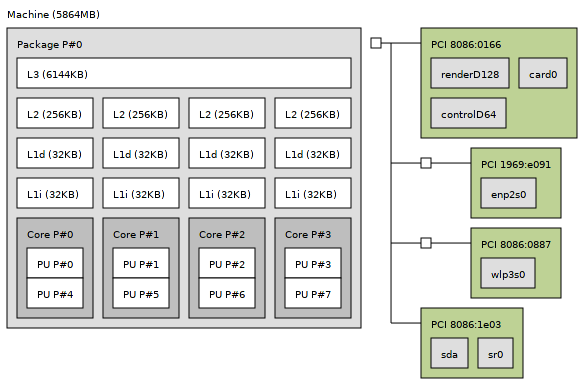
\includegraphics[width=100mm]{MEDIA/Topo.png}
        \caption{Caractéristiques de la machine utilisé}
    \end{figure}
\lstinputlisting{../kernel.c}

Notre boucle a besoin de 3 tableaux de taille n et d'un tableau de taille n$\times$n.\\
Chaque case du tableau prend 4 octets (int32\_t/float)\\
Le coût total en mêmoire est donc de $4n^2+12n$ octets.\\

Le cache L1 fait 32Ko, il faut donc prendre des tableaux de 85 cases. Coût total: 29.920 Ko

Le cache L2 fait 256Ko, il faut donc prendre des tableaux de 238 cases. Coût total: 229.432 Ko

Le cache L3 fait 6144Ko, il faut donc prendre des tableaux de 865 cases. Coût total: 3 003.280 Ko

Pour la RAM, nous prenons des tableaux de 2120 cases: coût total 18 003.04 Ko.

\begin{tabular}{ l c | c c }
    Type de Mémoire & Taille Mémoire & Taille Tableau & Coût Total\\\hline
    L1 & 32Ko & 85 & 29.920 Ko\\ 
    L2 & 256Ko & 238 & 229.432 Ko \\
    L3 & 6 144Ko & 865 & 3 033.280 Ko \\
    RAM & 5 864Mo & 2120 & 18.00304 Mo \\
\end{tabular}

\subsection*{Carastéristiques de la machine}

Hardware
\begin{itemize}
    \item{- I7 3630QM (~Fin 2012) :}
    \item{- 4 cores - 8 threads}
    \item{- Freq : ~2.4Ghz (Idle 1.2Ghz - Turbo mode 3.40 Ghz )}
    \item{- 6 Go de RAM }
\end{itemize}

Système
\begin{itemize}
    \item{- gcc 6.3.1}
    \item{- Arch x86\_64 ( noyaux Linux 4.10.6-1 Arch )}
\end{itemize}

\subsection*{Warmup}



Pour determiner le nombre de cycles de warmup nécessaires: On lance plusieurs fois la boucle de warmup, et l'on trace le graphe du temps d'éxécution en fonction du nombre de répétitons successives.

On sépare les cas pour les différent tailles de données:
\newpage
    \begin{figure}[ht!]
        \centering
        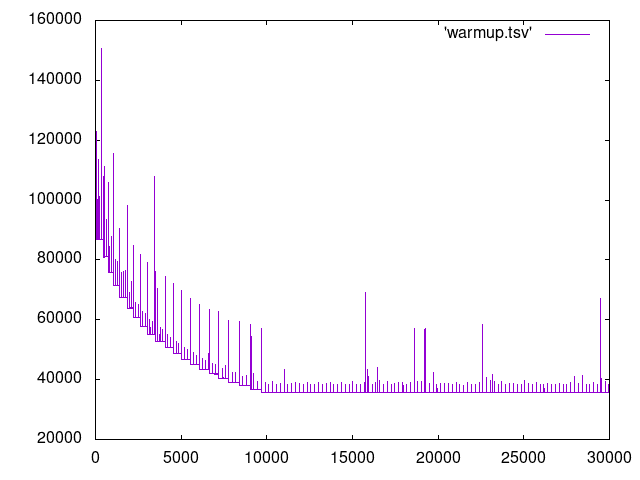
\includegraphics[width=120mm]{MEDIA/warmupL1_Cstate.png}
        \caption{Warmup en cache L1 avec tout Cstate autorisé}
    \end{figure}

On remarque que le warmup est relativement long, en désactivant les Cstates,celui-ci devient plus court.\\

En effet, les Cstates permettent d'économier l'énergie consommée par le processeur en endormant certains composants, qui peuvent être longs a réveiller.\\

Sans Cstates, le proceseur n'a que 3 états: Idle, Normal et Turbo, et passe donc très rapidement en mode turbo.\\
\newpage
    \begin{figure}[ht!]
        \centering
        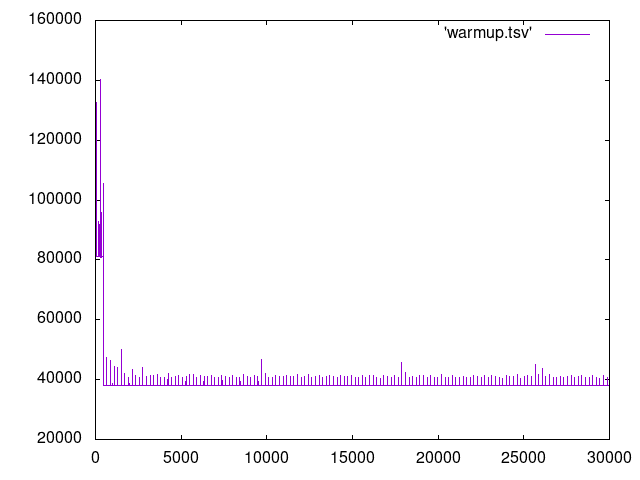
\includegraphics[width=120mm]{MEDIA/warmupL1_NOCstate.png}
        \caption{Warmup en cache L1 avec Cstate max=0}
    \end{figure}

Il nous faut donc 2000 cycles de warmup pour une taille de données retrant en cache L1.\\

Pour la suite, nous continuons a faire nos calculs avec Cstate max=0
\newpage
    \begin{figure}[ht!]
        \centering
        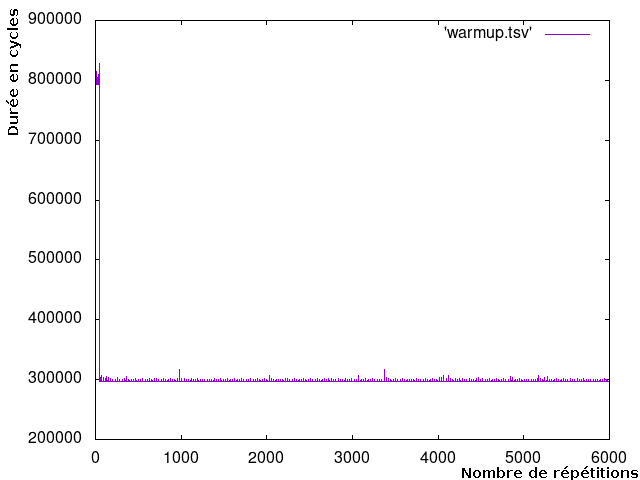
\includegraphics[width=120mm]{MEDIA/warmupL2_NOCstate.png}
        \caption{Warmup en cache L2}
    \end{figure}

On constate que les temps de calculs deviennent rapidement stables.

\newpage
    \begin{figure}[ht!]
        \centering
        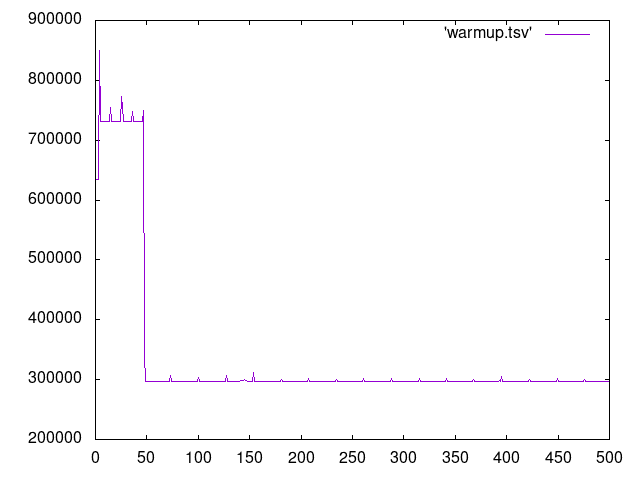
\includegraphics[width=120mm]{MEDIA/closeup.png}
        \caption{Warmup en cache L2}
    \end{figure}

    On décide de prendre 500 cycles de warmup pour avoir une marge.

\newpage 
    \begin{figure}[ht!]
        \centering
        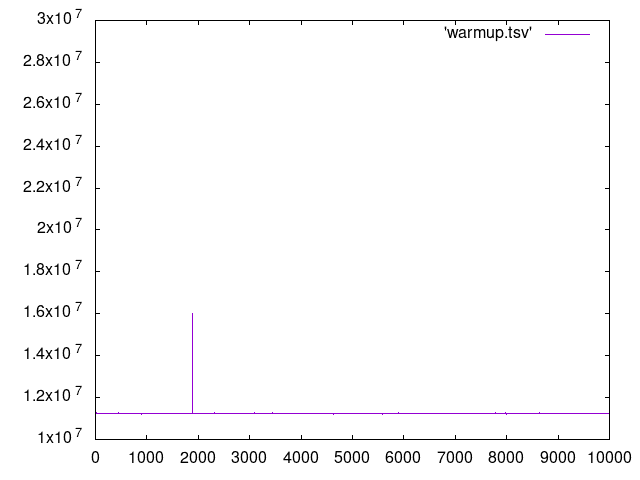
\includegraphics[width=120mm]{MEDIA/warmupL3_NOCstate.png}
        \caption{Warmup en cache L3}
    \end{figure}

Au niveau du L3, Nous avons commencé par tester pour 10 000 éxécutions. 

\newpage 
    \begin{figure}[ht!]
        \centering
        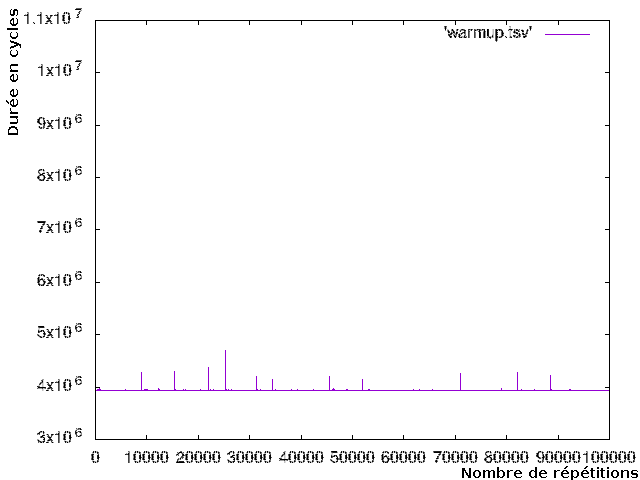
\includegraphics[width=120mm]{MEDIA/warmupL3_100000.png}
        \caption{Warmup en cache L3 }
    \end{figure}

On remarque, que pour 100 000 éxécutions, le programme finit plus vite a cahque fois!
On décide donc de tester pour 200 000 éxécutions 

\newpage
    \begin{figure}[ht!]
        \centering
        
\includegraphics[width=120mm]{MEDIA/warmupL3_200000.png}
        \caption{Warmup en cache L3 }
    \end{figure}

    On constate que pour les ~30K premières éxécutions, le temps de calcul est le même que pour chaqu'une des 10 000. Il descend ensuite a la valuer obtenue en pour chaque boucle des 100 000 tours de warmup.
-    \begin{figure}[ht!]
        \centering
        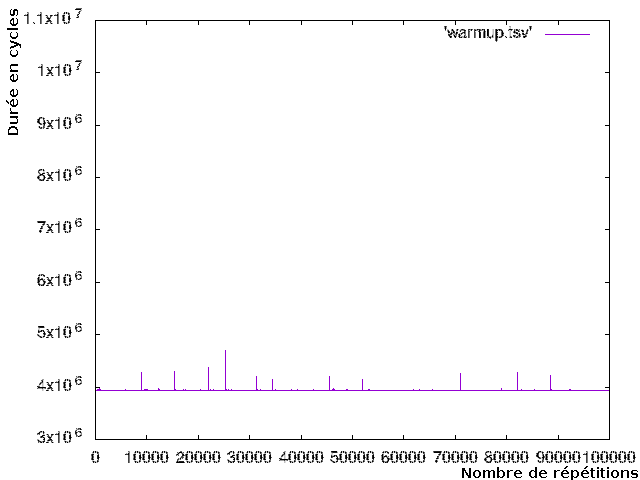
\includegraphics[width=120mm]{MEDIA/warmupL3_100000.png}
        \caption{Warmup en cache L3 }
    \end{figure}> méta-répétitions

->likwid(taille cache/tableaux)
->qualité code.





\end{document}
